% Main source file

\documentclass[a4paper,11pt]{book}
\usepackage[UKenglish]{babel}
\usepackage[T1]{fontenc}
\usepackage[latin1]{inputenc}
\usepackage{graphicx}
\usepackage{calc}
\usepackage{amsmath}
%\usepackage{hyperref}
\usepackage{natbib}
	
% Stuff that might be useful depending on individual needs
\usepackage{array}
\usepackage{boxedminipage}
\usepackage{rotating}
\usepackage{amssymb}
\usepackage{subfigure}
\usepackage{hhline}
\usepackage{moreverb}
\usepackage{float} 

%DIN TITTEL HER:
\newcommand{\mintittel}{NO TITLE}
\title{\mintittel}
\author{TOR-ANDREAS S. BJONE}
\date{\today}

% Setting for layout
\setlength{\textwidth}{14.5cm}
\setlength{\headheight}{13.6pt}
\setlength{\marginparwidth}{0.7cm}
%\setlength{\marginparsep}{0.7cm}
\setlength{\evensidemargin}{1cm}

% Fancy heading -  if you want it
\usepackage{fancyhdr}
\pagestyle{fancyplain}
\addtolength{\headwidth}{\marginparsep}
\addtolength{\headwidth}{\marginparwidth}
\renewcommand{\chaptermark}[1]%
	{\markboth{#1}{}}
\renewcommand{\sectionmark}[1]%
	{\markright{\thesection\ #1}}
\lhead[\fancyplain{}{\bfseries\thepage}]%
	{\fancyplain{}{\bfseries\rightmark}}
\rhead[\fancyplain{}{\bfseries\leftmark}]%
	{\fancyplain{}{\bfseries\thepage}}
\cfoot{}

% Below: depends on package float
% -----------------------------------------------------
% Definitions for algorithms
\floatstyle{boxed}
\newfloat{algorithm}{hbt}{loa}[chapter]
\floatname{algorithm}{Algorithm}

%\setcounter{secnumdepth}{3}
%New commands;

\renewcommand{\H}{\mathcal{H}}
\newcommand{\phid}{\dot{\phi}}
\newcommand{\phidd}{\ddot{\phi}}
\newcommand{\Phid}{\dot{\Phi}}
\newcommand{\Phidd}{\ddot{\Phi}}
\newcommand{\psid}{\dot{\psi}}
\newcommand{\Psid}{\dot{\Psi}}
\newcommand{\Psidd}{\ddot{\Psi}}
\newcommand{\R}{\mathcal{R}}
\renewcommand{\L}{\mathcal{L}}
\newcommand{\Rd}{\dot{\mathcal{R}}}
\newcommand{\M}{m_{Pl}}
\newcommand{\g}{g_{\mu\nu}}
\newcommand{\gu}{g^{\mu\nu}}
\newcommand{\Ricci}{R_{\mu\nu}}
\newcommand{\G}{G_{\mu\nu}}
\newcommand{\addotoa}{\dfrac{\ddot{a}}{a}}
\renewcommand{\dh}{\dot{h}}
\newcommand{\ddh}{\ddot{h}}
\newcommand{\dF}{\dot{F}}
\newcommand{\ddF}{\ddot{F}}
\newcommand{\dFoF}{\dfrac{\dF}{F}}
\newcommand{\ddFoF}{\dfrac{\ddF}{F}}
\newcommand{\synch}{\left(\delta_{ij}+h_{ij}\right)}
%\newcommand{\Chr}[2]{\Gamma_{#1}^{#2}


\newcommand{\tphi}{\tilde{\phi}}
\newcommand{\tpsi}{\tilde{\psi}}
\newcommand{\tdpsi}{\dot{\tilde{\psi}}}
\newcommand{\tPhi}{\tilde{\Phi}}
\newcommand{\tdPhi}{\dot{\tilde{\Phi}}}
\newcommand{\tPsi}{\tilde{\Psi}}
\newcommand{\tdPsi}{\dot{\tilde{\Psi}}}
\newcommand{\tE}{\tilde{E}}
\newcommand{\tB}{\tilde{B}}
\newcommand{\tg}{\tilde{g}}
\newcommand{\tV}{\tilde{V}}
\newcommand{\tT}{\tilde{T}}
\newcommand{\tNabla}{\tilde{\nabla}}
\newcommand{\tR}{\tilde{\rho}}
\newcommand{\ta}{\tilde{a}}
\newcommand{\trho}{\tilde{\rho}}
\newcommand{\tP}{\tilde{p}}
\newcommand{\tp}{\tilde{p}}
\newcommand{\tz}{\tilde{z}}
\newcommand{\teta}{\tilde{\eta}}
\renewcommand{\th}{\tilde{h}}
\newcommand{\tH}{\tilde{\mathcal{H}}}
\newcommand{\tdelta}{\tilde{\delta}}
\newcommand{\tv}{\tilde{v}}
\newcommand{\tw}{\tilde{w}}
\newcommand{\taddotoa}{\dfrac{\ddot{\ta}}{\ta}}
\newcommand{\tsynch}{\left(\delta_{ij}+\th_{ij}\right)}
\newcommand{\tOmega}{\tilde{\Omega}}
\newcommand{\C}{\mathcal{C}}

\newcommand{\tabb}[1]{Table \ref{#1}}
\newcommand{\fig}[1]{Figure \ref{#1}}
\newcommand{\eq}[1]{equation (\ref{#1})}
\newcommand{\chap}[1]{Chapter \ref{#1}}
\renewcommand{\sec}[1]{\S\ref{#1}}
\newcommand{\eqs}[2]{equations \eqref{#1} - \eqref{#2}}
\renewcommand{\t}[1]{\mathrm{#1}}
\renewcommand{\k}{{\boldsymbol{k}}}
\newcommand{\K}{(k_1+k_2+k_3)}
%\renewcommand{\sum}{\displaystyle\sum}

\newcommand{\be}{\begin{equation}}
\newcommand{\ee}{\end{equation}}
\newcommand{\ba}{\begin{align}}
\newcommand{\ea}{\end{align}}
\newcommand{\I}{\Bigg|}
\newcommand{\bea}{\begin{eqnarray}}
\newcommand{\eea}{\end{eqnarray}}
\newcommand{\bdm}{\begin{displaymath}}
\newcommand{\edm}{\end{displaymath}}
\newcommand{\beas}{\begin{eqnarray*}}
\newcommand{\eeas}{\end{eqnarray*}}

\newcommand{\khv}{\hat{\mathbf{k}}}
\newcommand{\nhv}{\hat{\mathbf{n}}}
\newcommand{\kh}{\hat{k}}

\newcommand{\av}[1]{\left< #1\right>}
\newcommand{\kv}{\mathbf{k}}
\newcommand{\kdv}{\mathbf{k}'}
\newcommand{\pv}{\mathbf{p}}
\newcommand{\pdv}{\mathbf{p}'}
\newcommand{\qv}{\mathbf{q}}
\newcommand{\qdv}{\mathbf{q}'}
\newcommand{\kmkd}{\mathbf{k}-\mathbf{k}'}
\newcommand{\pmpd}{\mathbf{p}-\mathbf{p}'}
\newcommand{\qmqd}{\mathbf{q}-\mathbf{q}'}
\newcommand{\ppkd}{\mathbf{p}+\mathbf{k}'}
\newcommand{\qpkd}{\mathbf{q}+\mathbf{k}'}
\newcommand{\Pow}[1]{\mathcal{P}\left(#1\right)}
\newcommand{\Pro}[3]{P_{#1 #2}\left( #3\right)}
\newcommand{\dk}{\frac{d^3\kv}{(2\pi)^3}}
\newcommand{\dkd}{\frac{d^3\kv'}{(2\pi)^3}}

% Einstein frame quantities

\newcommand{\tq}{\tilde{q}}
\newcommand{\tpi}{\tilde{\pi}}
\newcommand{\tDelta}{\tilde{\Delta}}

\newcommand{\cssq}{c_s^{\phantom{s}2}}
\newcommand{\tcssq}{\tilde{c}_s^{\phantom{s}2}}
%Fixing height of tables
\renewcommand{\arraystretch}{1.8}

%Wigner symbols
\newcommand{\wignertre}[2]{\genfrac{(}{)}{0pt}{}{#1}{#2}}
\newcommand{\wignersix}[2]{\genfrac{\{}{\}}{0pt}{}{#1}{#2}}
%============================================================
\begin{document}
\pagenumbering{roman}
%\pagestyle{plain}
\begin{titlepage}
\begin{center}

\bfseries
\huge%\LARGE
\mintittel

\vspace{2cm}
\LARGE
TOR-ANDREAS S. BJONE


\vspace{1cm}
\begin{figure}[h]
\centering

\includegraphics[width=7cm]{uiologo.eps}
\centering
\end{figure}
\vspace{3cm}
\Large
Thesis submitted for the degree of \\
Master of Science in Astronomy%Master of Science Thesis by\\
%\Large
%Amir Hammami\\

\vspace{0.8cm}
\large
Institute of Theoretical Astrophysics\\
University of Oslo

\vspace{0.8cm}
NO DATE

\end{center}
\normalfont

\end{titlepage}

\vspace*{18cm}
\noindent Copyright \copyright$\,$ 2024, TOR-ANDREAS S. BJONE 
\vspace{4mm}

\noindent This work, entitled ``\mintittel'' is distributed under the
terms of the Public Library of Science Open Access License, a copy of which can be found at
http://www.publiclibraryofscience.org. 

\chapter*{Abstract}
\addcontentsline{toc}{chapter}{\numberline{}Abstract}


\chapter*{Acknowledgments}
\addcontentsline{toc}{chapter}{\numberline{}Acknowledgments}

%\addcontentsline{toc}{chapter}{\numberline{}Contents}
\tableofcontents

\addcontentsline{toc}{chapter}{\numberline{}List of Figures}
\listoffigures
\newpage
\thispagestyle{empty}
\mbox{}

\newpage
\pagestyle{fancyplain}
\pagenumbering{arabic}


%Her har jeg kommentert ut mine delkapitler, denne malen fungerer slik at jeg har ett hoveddokument, som heter main.tex. I denne har jeg \include{navn på en annen .tex fil jeg ønsker at skal bli en del
% av dette dokumentet}. Dvs at i mitt tilfelle hadde jeg en main.tex, sammen med introduction.tex, cosmology.tex, fRgrav.tex osv.

\chapter{Introduction}

\include{background_theory}
\chapter{Theory}
\section{Background Theory}
\subsection{Theory about the Sun}
In the current state of solar modeling it is believed that the sun is composed stratified layers. The solar core, a hot and dense region that provides most of the energy produced by the sun by fusion

\citep{1996Sci...272.1286C}


where fusion produces energy
of a solar core, a radiative zone, a convective zone and an atmosphere


Statification
Radiative zone, superadiabaticity
Convection zone
Convective cells, granule size
Pressure scale height
Time scales


\section{Anelastic MHD}
\subsection{Anelastic model background}
Some of the MLT and pertubation theory here. Maybe derivation of continuity eq.
\subsection{General anelastic MHD}

In Mixing Length Theory (MLT) one looks at the characteristic mixing length $l_m$. This is the distance a parcel of fluid with thermodynamical properties different than the thermodynamical properties of the background will rise or fall before mixing with it's enviroments \citep{1925ZaMM....5..136P}. This model gives us the dominant balance for the lowest order equations and the relative sizes of pertubations to the first order \citep{1999ApJS..121..247L} and has been tested against fully-compressibile models, supporting it's validity \citep{1989ApJ...336.1022C}. 

This can be used to set up a thermodynamic background state on which you can use pertubation theory to set up a first order foreground which carries convection, under the assumption that we can describe convection as a pertubation upon a static background. In pertubation theory we say that an $\epsilon$-expanded variable can be written as $f=f_0+\epsilon f_1+\epsilon^2 f_2+...$, where $f_0$ is the zero-order term, $f_1$ is the first order and so on, and $\epsilon$ is a small pertubation parameter. From MLT we have that the velocity should be $\epsilon^{1/2}$-expanded, while the other thermodynamical variables should be $\epsilon$-expanded. Then the velocity $\mathbf{v}=\mathbf{v}_0 + \epsilon^{1/2}\mathbf{v}_1+\epsilon^{3/2}\mathbf{v}_2+...$ and the density $\rho=\rho_0+\epsilon\rho_1+\epsilon^2\rho_2+...$. We only look at the the zero- and first-order pertubations for the anelastic model. This expansion can be done for all the other thermodynamical variables but are shown here for velocity and density to derive the anelastic continuity equation. Since we will be working with a static background model in hydrostatic equilibrium we will set the background velocity to zero. We have that the continuity equation is 

\begin{equation}
    \frac{\partial\rho}{\partial t} = -\nabla\cdot (\rho\mathbf{v}).
\end{equation}
Plugging in the pertubed variables we get

\begin{equation}
    \epsilon\frac{\partial\rho_1}{\partial t} = -\nabla\cdot (\epsilon^{1/2}\rho_0\mathbf{v}_1+\epsilon^{3/2}\rho_1\mathbf{v}_1),
\end{equation}
where we used the fact that $\rho_0$ is not time-dependent. We look at the lowest non-vanishing velocity term and get the \textbf{continuity equation} for the anelastic model
\begin{equation}\label{eq:continuity}
    O(\epsilon^{1/2}):\ \nabla\cdot(\rho_0\mathbf{v})=0,
\end{equation}
setting $\mathbf{v}\equiv\mathbf{v}_1$ since the only velocity we look at is the first order pertubation. In a similar fashion one can derive all other MHD equations as have been done in \citep{1999ApJS..121..247L}. We will show the $\epsilon$-order as in this paper, but follow the notation of \citep{2021LRSP...18....5F} since we are not using scaled variables. In the following we let $x$ and $y$ be the horizontal directions and $z$ be the vertical upward direction so that the gravity $\mathbf{g}=-g\mathbf{\hat{k}}$. The pertubed entropy $s_1$, pressure $p_1$, temperature $T_1$, velocity $\mathbf{v}$ and density $\rho_1$ are functions of $(x,y,z,t)$ while the background entropy $s_0$, $p_0$, $T_0$ and $\rho_0$ are variables of only $z$. We then get that the \textbf{conservation of momentum} is
\begin{align}\label{eq:momentum}
    O(1):\ \frac{d\rho_0}{dz}=-\rho_0 g,\\
    O(\epsilon):\ \rho_0\left[\frac{\partial\mathbf{v}}{\partial t}+(\mathbf{v}\cdot\nabla)\mathbf{v}\right]=-\nabla p_1 + \rho_1\mathbf{g}+\frac{1}{4\pi}(\nabla\times\mathbf{B})\times\mathbf{B}+\nabla\cdot\mathbf{\Pi},
\end{align}
where $\mathbf{B}$ is the magnetic field and $\mathbf{\Pi}$ is the viscous stress tensor. The \textbf{conservation of entropy}
\begin{align}\label{eq:entropy_full}
    O(\epsilon^{1/2}):\ s_0=\text{const},\\
    O(\epsilon^{3/2}):\ \rho_0 T_0 \left[\frac{\partial s_1}{\partial t} + (\mathbf{v}\cdot \nabla)(s_0+s_1) \right]
    = \nabla\cdot(K\rho_0T_0\nabla s_1) + \frac{1}{4\pi}\eta \left| \nabla\times\mathbf{B} \right|^2+\left(\mathbf{\Pi}\cdot\nabla \right)\cdot\mathbf{v},
\end{align}
where $K$ and $\eta$ are the magnetic and thermal diffusivty respectively. The MHD \textbf{Ohm's law}
\begin{equation}\label{eq:ohms_law}
    O(\epsilon):\ \frac{\partial\mathbf{B}}{\partial t} = \nabla\times(\mathbf{v}\times\mathbf{B})-\nabla\times(\eta\nabla\times\mathbf{B}),
\end{equation}
with initial conditions
\begin{equation}
    \nabla\cdot\mathbf{B}=0
\end{equation}
For the \textbf{equation of state} we will assume an ideal gas and get
\begin{align}\label{eq:equation_of_state}
    O(1):\ p_0=r_*\rho_0T_0,\\
    O(\epsilon):\ \frac{\rho_1}{\rho_0}=\frac{p_1}{p_0}-\frac{T_1}{T_0},
\end{align}
where the spesific gas constant
\begin{equation}
    r_* = \frac{k_B}{\mu m_u},
\end{equation}
where $k_B$ is Boltzmanns constant, $\mu$ is the mean molecular weight and $m_u$ is the atomic mass unit. Lastly we get the \textbf{first law of thermodynamics}
\begin{align}\label{eq:first_law_thermodynamics}
    O(1):\ \frac{dT_0}{dz} = \frac{g}{c_p},\\
    O(\epsilon):\ \frac{s_1}{c_p} = \frac{T_1}{T_0}-\frac{p_1}{p_0},
\end{align}
where the spesific heat at constant pressure is
\begin{equation}
    c_p = \frac{r_*}{1-1/\gamma},
\end{equation}
and $\gamma$ is the adiabatic gas parameter ($5/3$ for a monoatomic ideal gas).

The main benefit of the anelastic approximation is that it filters out fast moving sound waves. This means that we can have a higher temporal resolution because we dont have to consider acoustic time scales, but instead only having to consider the much lower dynamic time scale, which is determined by the flow velocity and Alfvén speed. The reason the fast moving sound waves are filtered out will be shown in the following derivation.....

We now have equations for entropy \ref{eq:equation_of_state} \ref{eq:entropy_full}, velocity, temperature \ref{eq:first_law_thermodynamics}, density \ref{eq:equation_of_state} and the magnetic field \ref{eq:ohms_law}. To get an equation for the pressure we will take the the divergence of the momentum equation \ref{eq:momentum} and solve w.r.t. pressure. This gives an elliptic equation which can be solved by various numerical methods such as direct inversion or iterative methods.
\begin{equation*}
    \nabla^2 p_1 = \nabla\cdot(\rho_1\mathbf{g}) + \frac{1}{4\pi}\nabla\cdot\left[(\nabla\times\mathbf{B})\times\mathbf{B} \right]+\nabla^2\mathbf{\Pi}-\nabla\cdot\left[\frac{\partial(\rho_0\mathbf{v})}{\partial t} +\rho_0(\mathbf{v}\cdot\nabla)\mathbf{v}\right].
\end{equation*}
By Clairaut's theorem and the continuity equation \ref{eq:continuity} we get that $\nabla\cdot\partial_t(\rho_0\mathbf{v})=\partial_t\left[\nabla\cdot(\rho_0\mathbf{v})\right]=0$, giving us the \textbf{elliptic equation}

\begin{equation}\label{eq:elliptic}
    \nabla^2 p_1 = \nabla\cdot(\rho_1\mathbf{g}) + \frac{1}{4\pi}\nabla\cdot\left[(\nabla\times\mathbf{B})\times\mathbf{B} \right]+\nabla^2\mathbf{\Pi}-\nabla\cdot\left[\rho_0(\mathbf{v}\cdot\nabla)\mathbf{v}\right].
\end{equation}

\subsection{2D Ideal anelastic HD}
We start by looking at the simple problem where we have no magnetic field ($\mathbf{B}=0$), no viscous stress ($\mathbf{\Pi}=0$), no thermal diffusivty ($K=0$) and no $y$-dimension. This gives us the ideal form of our equations

\begin{align}
    \rho_0\left[\frac{\partial\mathbf{v}}{\partial t}+(\mathbf{v}\cdot\nabla)\mathbf{v}\right]=-\nabla p_1 + \rho_1\mathbf{g}\ &\text{(Momentum)},\\
    \left[\frac{\partial s_1}{\partial t} + (\mathbf{v}\cdot \nabla)(s_0+s_1) \right]
    = 0\ &\text{(Entropy)},\\
    \nabla^2 p_1 = \nabla\cdot(\rho_1\mathbf{g})-\nabla\cdot\left[\rho_0(\mathbf{v}\cdot\nabla)\mathbf{v}\right]\ &\text{(Elliptic)},
\end{align}
where $\mathbf{v}=v_x\mathbf{\hat{i}}+v_z\mathbf{\hat{k}}$. We can now write the conservation of momentum and entropy equations out w.r.t. the temporal derivatives, splitting the momentum equation into two equations for each direction. We start with the entropy equation and get

\begin{equation}\label{eq:ideal_entropy_wrt_t}
    \frac{\partial s_1}{\partial t} = - \left[ v_x \partial_x s_1 + v_z \partial_z s_1 + v_z\partial_z s_0 \right],
\end{equation}
where we used that $s_0$ is a variable of only $z$. Now the momentum equation

\begin{align}
    \mathbf{\hat{i}} &: \partial_t v_x = - \left[ v_x\partial_x v_x + v_z\partial_z v_y \right] - \frac{1}{\rho_0} \partial_x p_1,\\
    \mathbf{\hat{k}} &: \partial_t v_z = - \left[ v_x\partial_x v_z + v_z\partial_z v_z \right] - \frac{1}{\rho_0}\partial_z p_1 - \frac{\rho_1}{\rho_0} g.
\end{align}
And finally the elliptic equation

\begin{align*}
    \nabla^2 p_1 =&- \rho_0 [ v_x\partial_x^2 v_x + v_z\partial_z^2 v_z + \left( \partial_x v_x \right)^2 + \left( \partial_z v_z\right)^2\\
                   &+ 2\partial_x(v_z)\partial_z(v_x) + v_x\partial_x\partial_z v_z + v_z\partial_x\partial_z v_x]\\
                    &- \partial_z \left(\rho_0\right)\left[ v_x\partial_x v_z + v_z\partial_z v_z \right]
\end{align*}



\subsection{Adding thermal diffusivity}
\subsection{Adding viscous stress}

chrome-extension://efaidnbmnnnibpcajpcglclefindmkaj/https://arxiv.org/pdf/1408.3677.pdf

Single ion plasma:
\begin{equation}
    \mu_{ZZ} = 0.96 \frac{3}{4\sqrt{\pi}}\frac{\sqrt{M_Z} T_Z^{5/2}}{Z^4 e^4 \ln\Lambda_Z}
\end{equation}

where $\ln\Lambda_Z$ is the Columb logarithm. 
\href{chrome-extension://efaidnbmnnnibpcajpcglclefindmkaj/https://www.nrl.navy.mil/Portals/38/PDF%20Files/NRL_Plasma_Formulary_2019.pdf?ver=lSvX72q0HmFwRWJWBzaI6A%3d%3d&timestamp=1612555310291}{...}

Typically 10-20. We pick 10.


, $M_Z=m_u$ for Hydrogen, $Z=1$ for Hydrogen.




\subsection{Adding the magnetic field}

\section{Numerical Methods}
\subsection{Discretization and derivatives}

The simulation box is set up with $N_z$ grid points in the z-direction and $N_x$ in the x-direction. These have a resolution of $\Delta z$ and $\Delta x$ respectively. Then our grid points are at locations
\begin{align*}
    z_i &= z_0 + i\Delta z,\ i\in[0,N_z-1], \\ 
    x_j &= x_0 + j\Delta x,\ j\in[0,N_x-1].\\ 
\end{align*}
For the temporal discretization we get that the resolution $\Delta t$ will be different in each time-step due to the Courant-Friedrichs-Lewy (CFL) condition from the Von Neumann analysis. We start at a time $t_0$ and before ending at a time $T$. The time of at step $n+1$ is then
\begin{equation*}
    t_{n+1} = t_n + \Delta t
\end{equation*}
We name the foreground variables $f(z,x,t)$ and the background variables $h(z)$. These are then discretized as
\begin{align*}
    f(z,x,t) &\rightarrow f(z_i, x_i, t_n) = f_{i,j}^n,\\
    h(z) &\rightarrow h(z_i) = h_i.
\end{align*}
We then let the analytical derivatives go to a numerical derivative on the discretized variables, here for a derivative in the x-direction
\begin{equation*}
    \frac{\partial f(z,x,t)}{\partial x}\rightarrow \left[\frac{\partial f(z_i,x_j,t_n)}{\partial t} \right]_{i,j}^n.
\end{equation*}
These are handled using a number of known spacial and temporal schemes. For the temporal schemes we will use the Runge-Kutta methods and for the spacial methods we have to take care in which method used based on the form of the equation. As is shown in section \ref{subsec:von_neumann} from Von Neumann analysis the advection equation is numerically unstable for a variety of spacial schemes based on the order of the Runge-Kutta method. Especially the central schemes are unstable and the advection terms should therefore be handled using upwind methods, or forward spacial (FS). Using the second order upwind method we have
\begin{equation}
    \left[\frac{\partial f}{\partial x} \right]_{i,j}^n= 
    \begin{cases} 
        \frac{3f_{i,j}^n-4f_{i,j-1}^n+f_{i,j-2}^n}{2\Delta x} & \text{if } v_x \geq 0 \\
        \frac{-3f_{i,j}^n+4f_{i,j+1}^n-f_{i,j+2}^n}{2\Delta x} & \text{if } v_x < 0 
    \end{cases}
\end{equation}
In the following we will write out the momentum- and entropy-equations using the second order central scheme where possible and keep the brackets on derivatives including temporal methods or terms that needs an FS scheme.
\begin{align}
    \left[\frac{\partial v_x}{\partial t} \right]_{i,j}^n &= -\frac{1}{\rho_{0,(i)}}\frac{p_{1,(i,j+1)}^n - p_{1,(i,j-1)}^n}{2\Delta x} - v_{x,(i,j)}^n \left[\frac{\partial v_{x}}{\partial x}\right]_{i,j}^n - v_{z,(i,j)}^n \left[\frac{\partial v_{x}}{\partial z}\right]_{i,j}^n, \\
    \left[\frac{\partial v_z}{\partial t} \right]_{i,j}^n &= -\frac{1}{\rho_{0,(i)}}\frac{p_{1,(i+1,j)}^n - p_{1,(i-1,j)}^n}{2\Delta z} - v_{x,(i,j)}^n \left[\frac{\partial v_{z}}{\partial x}\right]_{i,j}^n - v_{z,(i,j)}^n \left[\frac{\partial v_{z}}{\partial z}\right]_{i,j}^n - \frac{\rho_{1,(i,j)}^n}{\rho_{0,(i)}}g(z_i)\\
    \left[\frac{\partial s_1}{\partial t}\right] &= - v_{x,(i,j)} \left[\frac{\partial s_1}{\partial x} \right]_{i,j}^n- v_{z,(i,j)} \left[\frac{\partial s_1}{\partial z} \right]_{i,j}^n - v_{z,(i,j)}\frac{s_{0,(i+1,j)}-s_{0,(i-1,j)}}{2\Delta x}. 
\end{align}

\subsection{The Elliptic Equation}

We call the right hand side of the elliptic equation \ref{eq:elliptic} for $F(t,z,x)$ and write the equation on discretized form
\begin{equation}
    \left[\nabla^2 p \right]_{i,j}^n = F_{i,j}^n.
\end{equation}
We remove the superscript, keeping in mind that this is the pertubed pressure at timestep $n$. Using the second order central second derivative we get that
\begin{equation}
    \frac{p_{i+1,j}-2p_{i,j}+p_{i-1,j}}{\Delta z^2} + \frac{p_{i,j+1}-2p_{i,j}+p_{i,j-1}}{\Delta x^2} = F_{i,j}.
\end{equation}
We call $a\equiv1/\Delta z^2$, $b\equiv1/\Delta x^2$ and $c\equiv-2(a+b)$. This gives us that

\begin{equation}
    ap_{i+1,j}+ap_{i-1,j}+cp_{i,j}+bp_{i,j+1}+bp_{i,j-1}=F_{i,j}
\end{equation}
This can then be solved for the pressure at $(i,j)$, giving

\begin{equation}
    p_{i,j} = \frac{F_{i,j} - a(p_{i+1,j} + p_{i-1,j}) - b(p_{i,j+1}+p_{j-1})}{c}
\end{equation}
To solve this we will use an iterative method....k+1, k. Show algo. Jacobi or Gauss-Seidel if we figure that out....
.....

.....

.....

\subsection{Stability Analysis}
\label{subsec:von_neumann}

We will use Von Neumann analysis of the advection equation to determine the required time-step sizes for our solver. The advection equation is
\begin{equation}
    \frac{\partial u(t,x)}{\partial t} = -a \frac{\partial u(t,x)}{\partial x},
\end{equation}
where $u(t,x)$ is the exact solution and $a$ is constant representing the velocity. This is discretized over a grid such that $y(t_n,x_j)=y_{n,j}$, where $t_n = n\Delta t$ and $x_j = j\Delta x$ for $n,j\in\mathbb{N}$, is our numerical solution. The advection equation then becomes

\begin{equation}
    \left[\frac{\partial y}{\partial t}\right]_{n,j} = -a \left[\frac{\partial y}{\partial x}\right]_{n,j}.
\end{equation}
The numerical solution is
\begin{equation}
    y_{n,j} = u(t_n,x_j)+\epsilon_{n,j},
\end{equation}
where $\epsilon_{n,j}$ is the round-off error. The round-off error must also satisfy the discretized equation and this gives us that
\begin{equation}\label{eq:advection_error}
    \left[\frac{\partial \epsilon}{\partial t}\right]_{n,j} = -a \left[\frac{\partial \epsilon}{\partial x}\right]_{n,j}.
\end{equation}
We expand the round-off error as a fourier series
\begin{equation}
    \epsilon(t_n,x_j) = \sum_m E_m(t_n) e^{i k_m j\Delta x},
\end{equation}
where $k_m$ is the wavenumber and $E_m(t_n)$ is the time-dependent amplitude of the error. When inserting this into our differential equation we get a linear difference equation, meaning that each of the terms behave like the entire series, so we can consider the growth of only one term
\begin{equation}
    \epsilon_m(t_n,x_j) = E_m(t_n) e^{i k_m j\Delta x}.
\end{equation}
We will show the calculations using the first-order upwind scheme with the second-order Runge-Kutta scheme. Since this should be true for any $m$ we remove the subscipt, define $\beta\equiv k\Delta x$ and get that the spacial derivative is
\begin{align*}
    \left[\frac{\partial \epsilon}{\partial x}\right]_{n,j} &= \frac{\epsilon_{n,j}-\epsilon_{n,j-1}}{\Delta x}\\
    &= \frac{E(t_n) e^{i \beta j}- E(t_n) e^{i \beta (j-1)}}{\Delta x}\\
    &= E(t_n)e^{i\beta j} \frac{1-e^{-i\beta}}{\Delta x}.
\end{align*}
This gives us that the advection equation \ref{eq:advection_error} becomes
\begin{align}
    \left[\frac{\partial \epsilon}{\partial t}\right]_{n,j} = e^{i\beta j}\left[\frac{\partial E(t_n)}{\partial t}\right]_{n,j} &= -a E(t_n)e^{i\beta j} \frac{1-e^{-i\beta}}{\Delta x}\\
    \left[\frac{\partial E(t_n)}{\partial t}\right]_{n,j} &= -a E(t_n)\frac{1-e^{-i\beta}}{\Delta x}.
\end{align}
We define $\lambda= - \frac{a}{\Delta x}\left( 1-e^{-i\beta} \right)$ which gives us 
\begin{equation}
    \mu = \Delta t \lambda = - C\left( 1-e^{-i\beta} \right),
\end{equation}
where $C\equiv a\Delta t/\Delta x$ is the Courant number. This means that the differential equation for the time-dependent error is
\begin{equation}
    \left[\frac{\partial E(t_n)}{\partial t}\right]_{n,j} = \lambda E_n.
\end{equation}
Using this with the second order Runge-Kutta scheme, the slopes for the time-dependent error is
\begin{align*}
    k_1 &= \lambda E_n,\\
    k_2 &= \lambda \left(E_n+\frac{\Delta t}{2}k_1 \right) = E_n \left( \lambda + \Delta t \lambda^2 \right).
\end{align*}
And the next time-step for the error is
\begin{align*}
    E_{n+1} &= E_n + \Delta t \left( \frac{k_1}{2} +\frac{k_2}{2} \right)\\
    &= E_n \left( 1 +\Delta t \lambda + \frac{1}{2}\left( \Delta t\lambda \right)^2 \right)\\
    & = E_n \left( 1 + \mu + \frac{1}{2}\mu^2  \right).
\end{align*}
This gives us the amplification factor 
\begin{equation}
    g = \frac{E_{n+1}}{E_n} = \left( 1 + \mu + \frac{1}{2}\mu^2  \right).
\end{equation}
We require $|g|\leq 1$, meaning that the time-dependent error does not grow in time. If this is any bigger than $1$ the error will grow exponentially, giving an unstable numerical solution. Following the same steps for some other schemes we get the following equations for spacial schemes:
\begin{align*}
    \text{First order upwind} &: \mu=-C\left(1-e^{-i\beta}\right),\\
    \text{Second order upwind} &: \mu=-\frac{C}{2}\left(3-4e^{-i\beta}+e^{-2i\beta}\right),\\
    \text{Second order central} &: \mu = -\frac{C}{2}\left(e^{i\beta} - e^{-i\beta}\right),\\
    \text{Fourth order central} &: \mu = - \frac{C}{12}\left(-e^{2i\beta}+8e^{i\beta}-8e^{-i\beta}+e^{-2i\beta}\right).
\end{align*}
And for the temporal schemes:
\begin{align*}
    \text{First order RK} &: g = 1+\mu,\\
    \text{Second order RK} &: g = 1+\mu + \frac{1}{2}\mu^2,\\
    \text{Third order RK} &: g = 1+\mu + \frac{1}{2}\mu^2+\frac{1}{6}\mu^3,\\
    \text{Fourth order RK} &: g = 1+\mu + \frac{1}{2}\mu^2+\frac{1}{6}\mu^3+\frac{1}{24}\mu^4.
\end{align*}
In figures \ref{fig:vn_rk1}, \ref{fig:vn_rk2}, \ref{fig:vn_rk3} and \ref{fig:vn_rk4} we see the amplification factor for different $C$ and $\beta$. Using the periodicity of $\beta$ we can pick $\Delta x$ and a corresponding $\Delta t$ given the magnitude of $a$.
\begin{figure}[htbp]
    \centering
    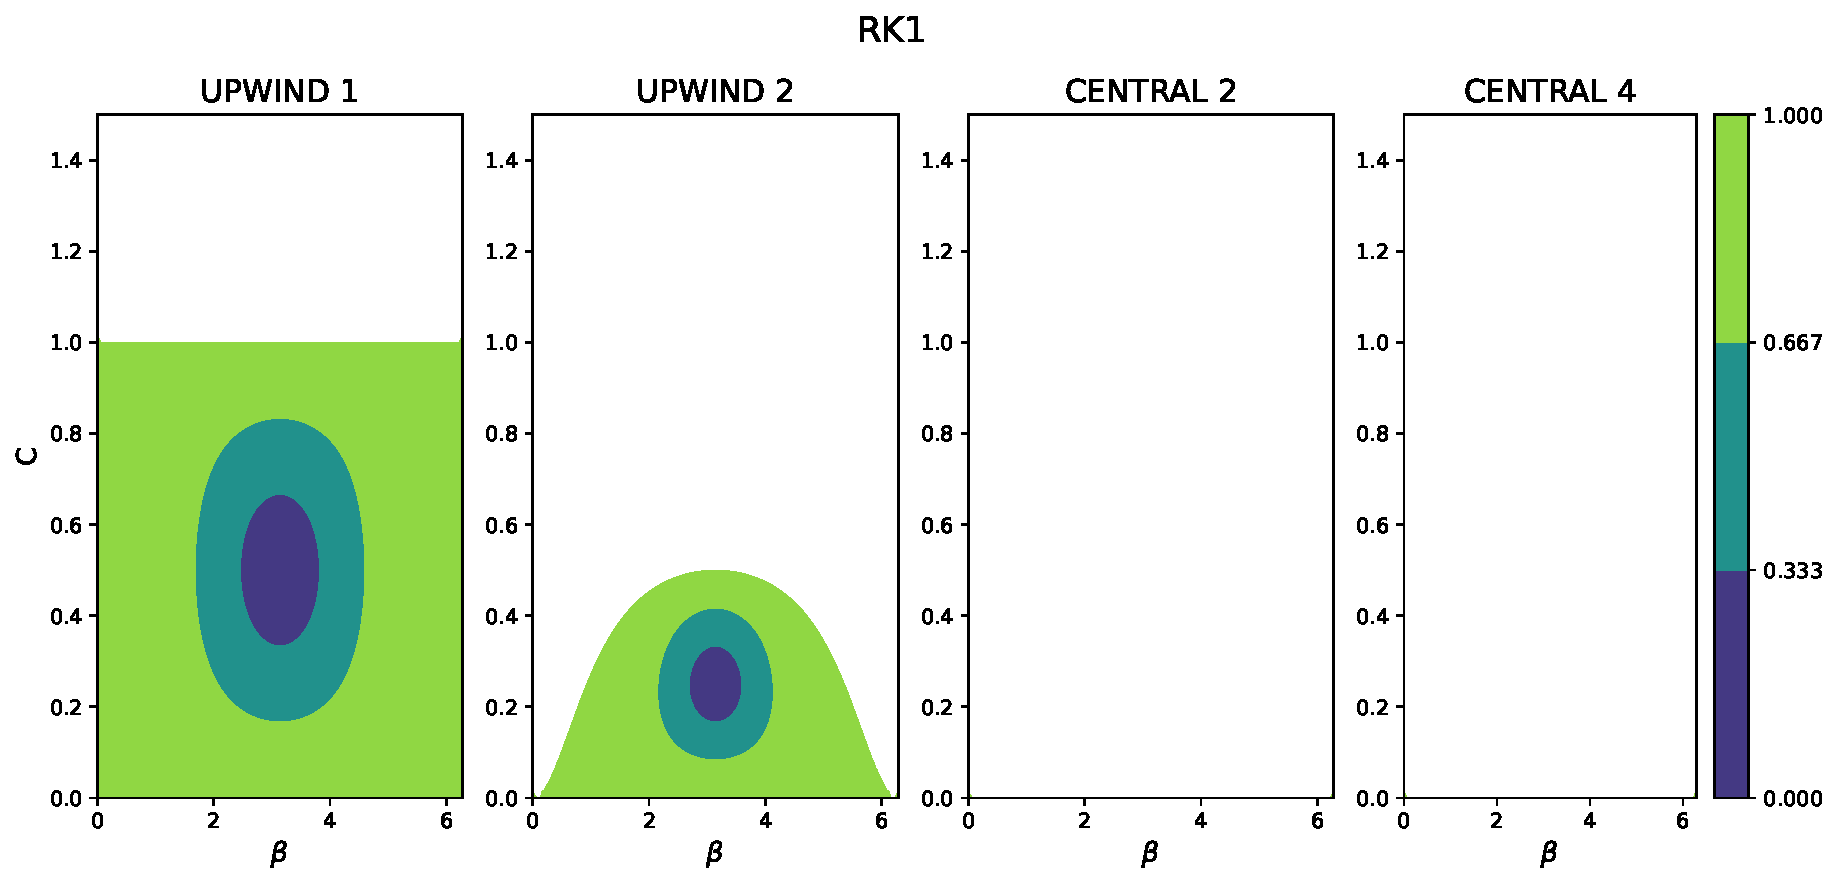
\includegraphics[width=0.8\linewidth]{./von_neumann_figs/vn_rk1.pdf} % Adjust the width as necessary
    \caption{Amplification factor magnitude for the first-order Runge Kutta scheme.}
    \label{fig:vn_rk1} % For referencing the figure elsewhere in your document
\end{figure}
\begin{figure}[htbp]
    \centering
    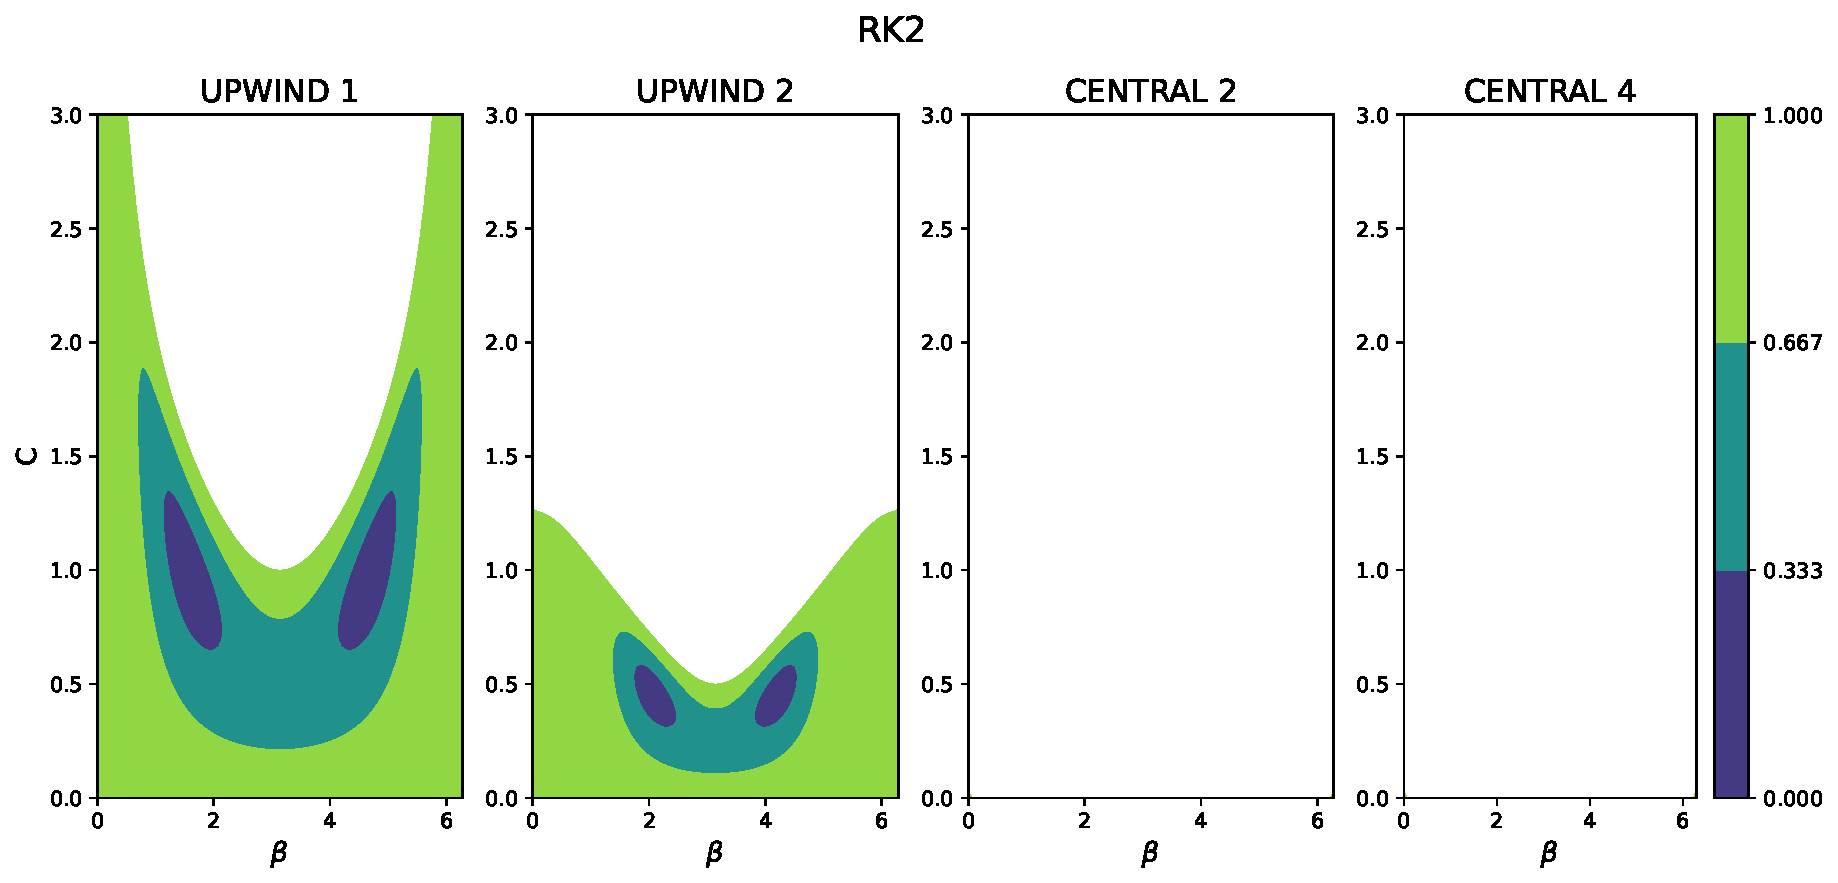
\includegraphics[width=0.8\linewidth]{./von_neumann_figs/vn_rk2.pdf} % Adjust the width as necessary
    \caption{Amplification factor magnitude for the second-order Runge Kutta scheme.}
    \label{fig:vn_rk2} % For referencing the figure elsewhere in your document
\end{figure}
\begin{figure}[htbp]
    \centering
    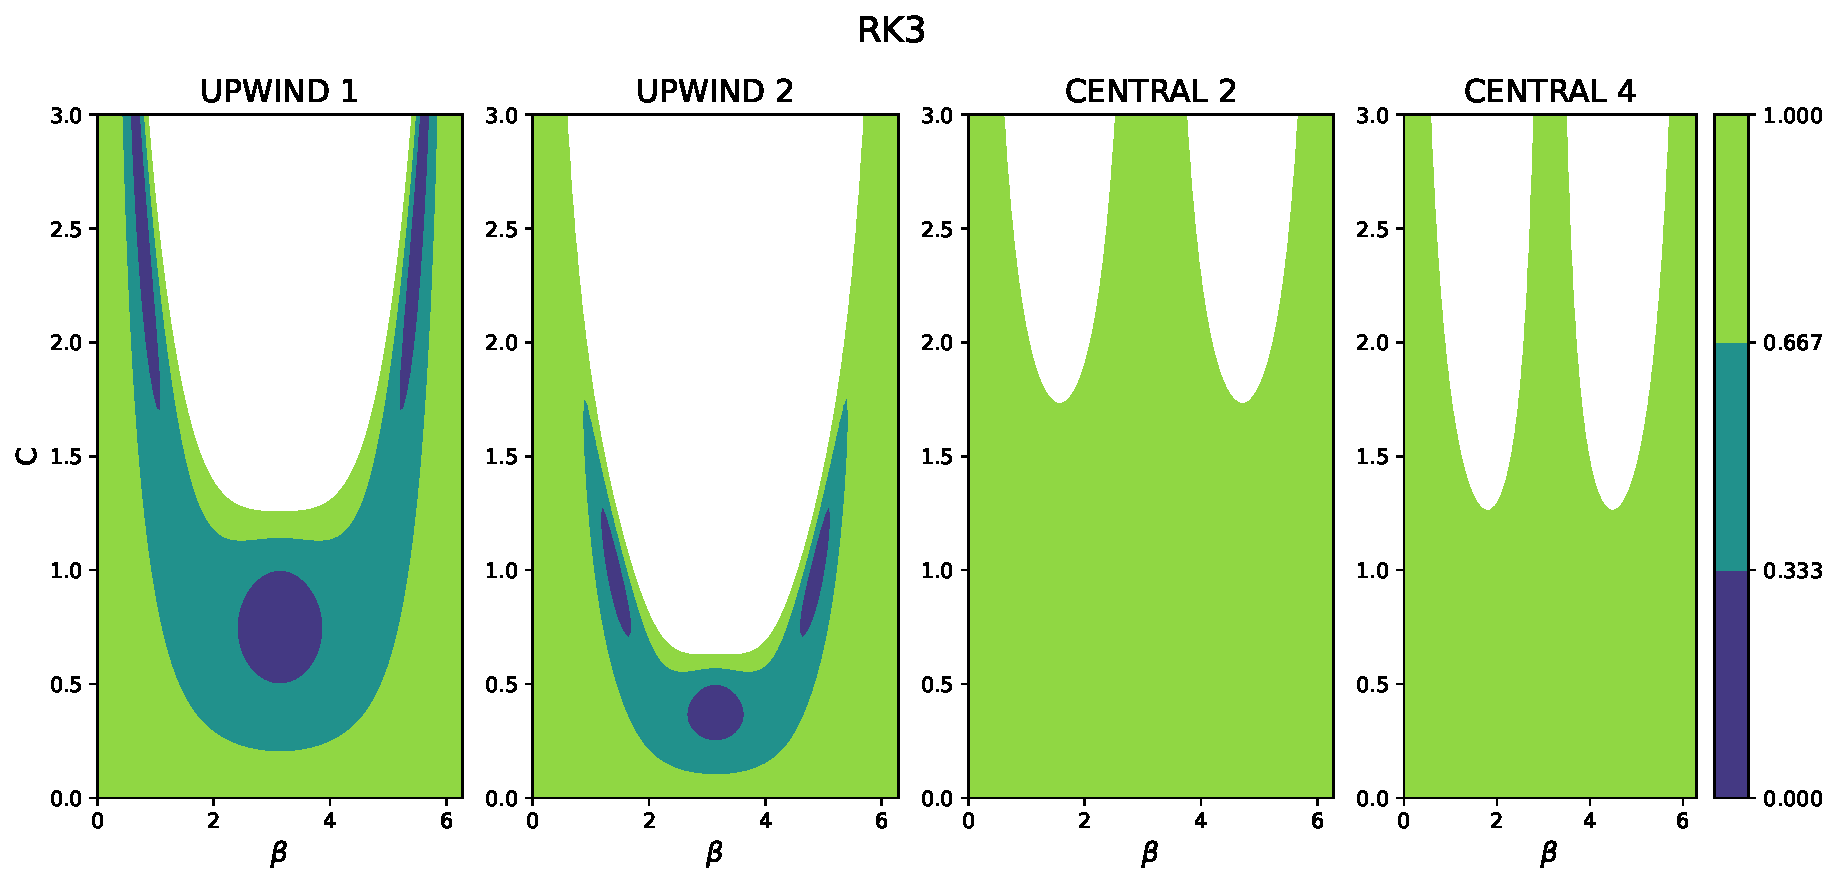
\includegraphics[width=0.8\linewidth]{./von_neumann_figs/vn_rk3.pdf} % Adjust the width as necessary
    \caption{Amplification factor magnitude for the third-order Runge Kutta scheme.}
    \label{fig:vn_rk3} % For referencing the figure elsewhere in your document
\end{figure}
\begin{figure}[htbp]
    \centering
    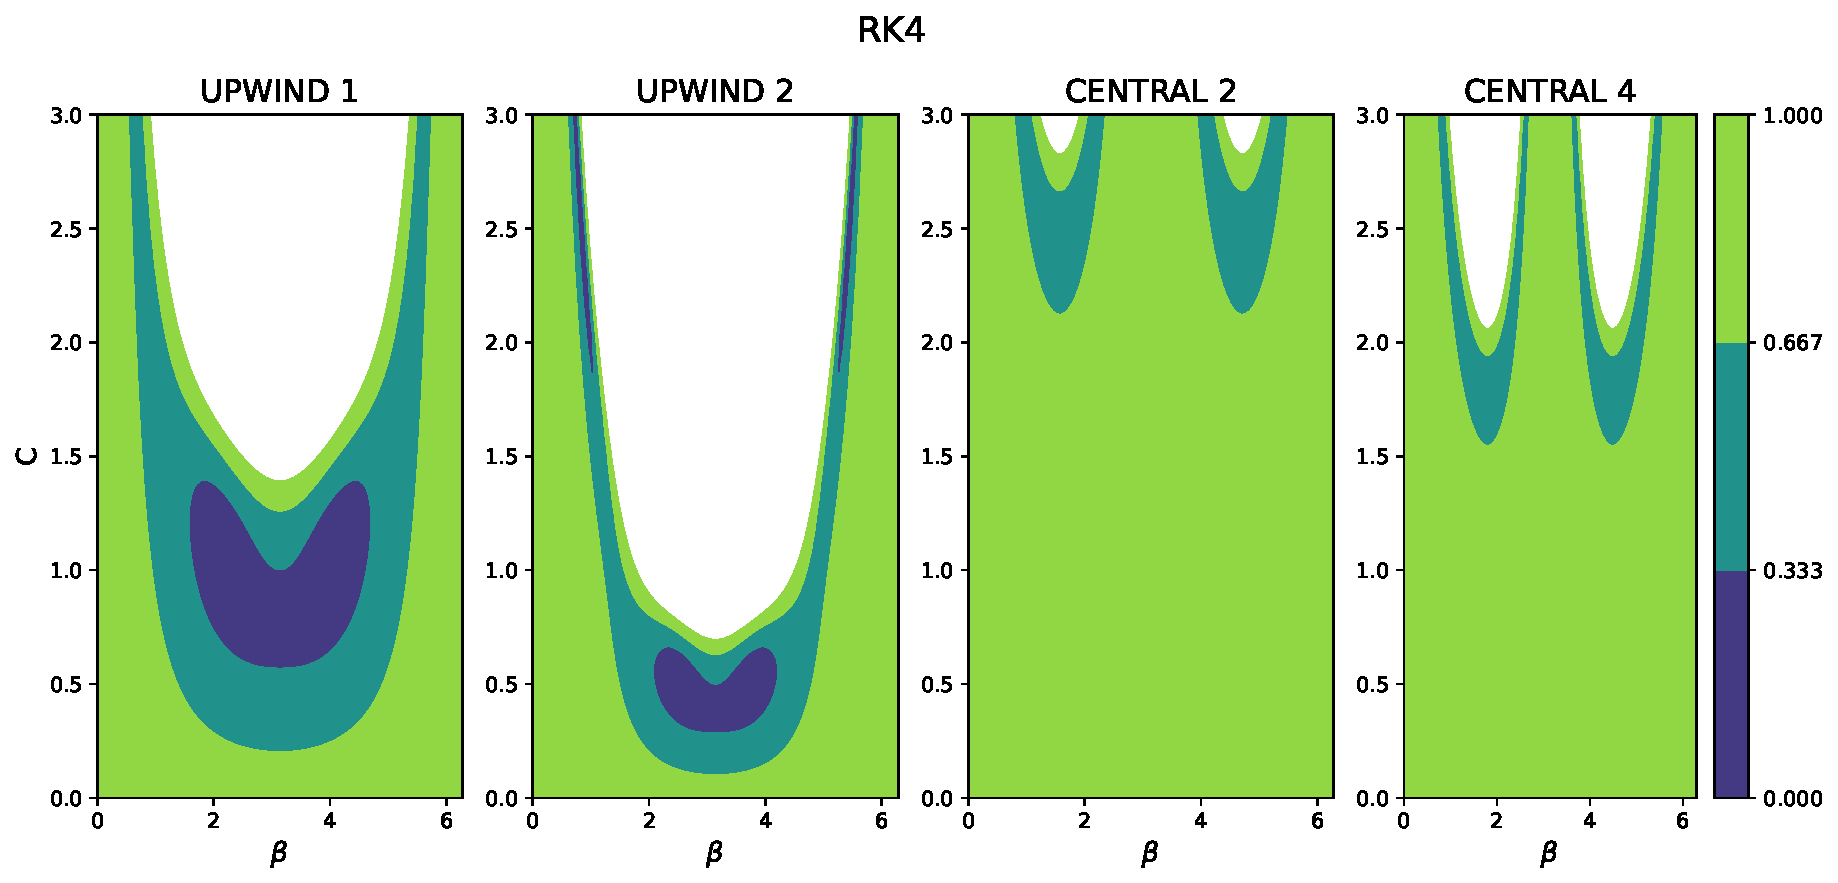
\includegraphics[width=0.8\linewidth]{./von_neumann_figs/vn_rk4.pdf} % Adjust the width as necessary
    \caption{Amplification factor magnitude for the fourth-order Runge Kutta scheme.}
    \label{fig:vn_rk4} % For referencing the figure elsewhere in your document
\end{figure}


\subsection{Background Initialization}

We base our background on reference values from the standard solar model, Solar S, \citep{1996Sci...272.1286C}. This data is downloaded from \href{https://users-phys.au.dk/~jcd/solar_models/cptrho.l5bi.d.15c}{https://users-phys.au.dk/~jcd/solar_models/cptrho.l5bi.d.15c} at 31.08.2023. The reference values for density $\rho_0(r_r)$, temperature $T_0(r_r)$ and pressure $p_0(r_r)$ are picked at a radius $r_r=0.71R_{\odot}$, which is the bottom of the convection zone \citep{1991ApJ...378..413C}. The mass at this point is calculated by
    \begin{equation}
        m(r_r)=\int_0^{r_r} dm = 4\pi \int_0^{r_r} \rho(r')r'^2 dr',
    \end{equation}
using cumulative trapezoidal integration. Having this we can use the following equations to integrate up and down from the reference point.

We are using an ideal gas model and therefore can not use this data as our entire background. This is because the temperature gradient of the background would not be large enough to produce convection numerically. Instead we will integrate out from our reference values and create a hydrostatic background. We will force convective instability by setting the superadiabaticity parameter 
    \begin{equation*}
        \Delta\nabla = \left(\frac{\partial\ln T}{\partial\ln p} \right)_{*} - \left(\frac{\partial\ln T}{\partial\ln p} \right)_{ad} = \nabla_{*} -\nabla_{ad} > 0,
    \end{equation*}
where $\nabla_{*}$ is the adiabatic temperature gradient of the star and $\nabla_{ad}=0.4$ is the adiabatic temperature gradient for an ideal gas. We therefore set 
    \begin{equation*}
    \nabla_{*} -\nabla_{ad} = 
        \begin{cases} 
        k & \text{if } r \geq 0.7 R_{\odot} \\
        0 & \text{if } r < 0.7 R_{\odot}
        \end{cases}
    \end{equation*}
For an ideal gas we have $\nabla_{ad}=0.4$ and we can then integrate our variables using the following equations.

\textbf{Mass of shell with thickness $dr$}
\begin{equation}\label{eq:mass_shell}
    \frac{dm}{dr} = 4\pi r^2\rho_0(r).
\end{equation}

\textbf{Hydrostatic equilibrium condition}
    \begin{equation}\label{eq:hydrostatic_equilibrium}
        \frac{dp_0}{dr} = -\frac{G m(r)}{r^2}\rho_0(r),
    \end{equation}
where $G$ is Newtons gravitational constant.

\textbf{????}
    \begin{equation}\label{eq:dT_dr}
        \frac{d T_0}{d r} = \nabla_{*} \frac{T_0}{p_0}\frac{d p_0}{d r}. 
    \end{equation}

We also have the \textbf{entropy gradient}
    \begin{equation*}
        \frac{ds}{dr} = -\frac{c_p}{H} \Delta\nabla,
    \end{equation*}
where the pressure scale height
    \begin{equation*}
        H = - \frac{dr}{d\ln p_0} = - p_0\frac{dr}{dp_0},
    \end{equation*}
the spesific heat capacity at constant pressure \citep{1999ApJS..121..247L}
    \begin{equation*}
        c_p = \frac{r_*}{1-1/\gamma},
    \end{equation*}
and $r_*$ is the spesific gas constant and $\gamma$ is the adiabatic parameter. The gas constant is taken from the ideal gas law on the from
    \begin{equation*}
        p = \frac{k_B}{\mu m_u} T,
    \end{equation*}
where $k_B$ is Boltzmanns constant $m_u$ is the atomic mass unit and $\mu$ is the mean molecular mass. Using the chemical abundaces of Hydrogen $\text{Ab(H)}=12$, Helium $\text{Ab(He)}=10.93$ and metals $\text{Ab(Metals)}=0.012$ \citep{2007SSRv..130..105G} we can calculate their relative number densities by 
    \begin{equation*}
        n_E = 10^{\text{Ab(E)}},
    \end{equation*}
the mass densities
    \begin{equation*}
        \rho_E = n_E\cdot m_E,
    \end{equation*}
where $m_e$ is the mass of the element, and the fractional abundance
    \begin{equation*}
        X_E = \frac{\rho_E}{\rho} = \frac{n_E m_E}{\sum_i n_i m_i},
    \end{equation*}
where $\rho$ is the total density. This gives us that $n_\text{H}=10^{12}$, $n_\text{He}=10^{10.93}$ and $n_\text{metals} = 10^{0.012}\approx1$. For simplification we firstly approximate $n_\text{metals}=0$, since $n_\text{metals}\approx1 \ll n_\text{H},n_\text{He}$, secondly $m_\text{He}\approx 4m_\text{H}$ and thirdly $m_\text{H}\approx m_u$. Then the the fractional abundance for Hydrogen, Helium and metals are
    \begin{align*}
        X_\text{H} &= \frac{n_\text{H}}{n_\text{H}+4 n_\text{He}} \approx 0.746,\\
        X_\text{He} &= \frac{4n_\text{He}}{n_\text{H}+4n_\text{He}}\approx 0.254, \\
        X_\text{metals} &= 1 - X_{\text{H}} - X_\text{He} \approx 0.000
    \end{align*}
We will assume full ionization due to the high temperatures and densities of the convection zone as can be seen in figures \ref{fig:temperature} and \ref{fig:pressure} from the standard solar model. Then the total number of particles due to Hydrogen is 
\begin{equation*}
    \frac{2X_\text{H}\rho}{m_u},
\end{equation*}
by one proton and electron. The total number of particles due to Helium is
\begin{equation*}
    \frac{3 X_\text{He}\rho}{4 m_u},
\end{equation*}
by one alpha particle and two electrons. Then the total number of particles
\begin{equation*}
    n_{total} = \frac{\rho}{m_u}\left( 2X_\text{H} + \frac{3 X_\text{He}}{4}{2} \right).
\end{equation*}
This gives us the mean molecular weight per particle
\begin{equation}
    \mu = \frac{1}{2X_\text{H} + 3X_\text{He}/4}\approx 0.594.
\end{equation}
We can then calculate the spesific gas constant 
    \begin{equation*}
        r_* = \frac{k_B}{m_u \mu},
    \end{equation*}
and the \textbf{entropy gradient}
    \begin{equation}\label{eq:entropy_gradient}
        \frac{ds}{dr} = p_0 \frac{k_B}{\mu m_u}\frac{\Delta\nabla}{1-1/\gamma}\frac{dp_0}{dr}.
    \end{equation}
We integrate this up to a radius $r_e$ and down to a radius $r_b$, limiting $dr$ for numerical stability. The limitation on $dr$ is implemented by picking a $p<1$ such that 
    \begin{equation*}
        dr = \frac{pV}{f},
    \end{equation*}
for a variable $V$ with
    \begin{equation*}
        f = \frac{dV}{dr}.
    \end{equation*}
This is done for all the variables and the smalles $dr$ is picked. For updating the density in each grid point we use the ideal gas \textbf{equation of state}
    \begin{equation}\label{eq:eos}
        \rho = \frac{p}{T}\frac{m_u \mu}{k_B}.
    \end{equation}

When we have the background set up we can interpolate this to a grid. We have done this using linear interpolation and the comparrison between our background model and the Solar S model from radius $r=0.6R_{\odot}$ to $0.97R_{\odot}$ can be seen in figures \ref{fig:temperature} for temperature, \ref{fig:pressure} for pressure, \ref{fig:density} for density and \ref{fig:gravitationa_acceleration} for gravitational acceleration.

\begin{figure}[htbp]
    \centering
    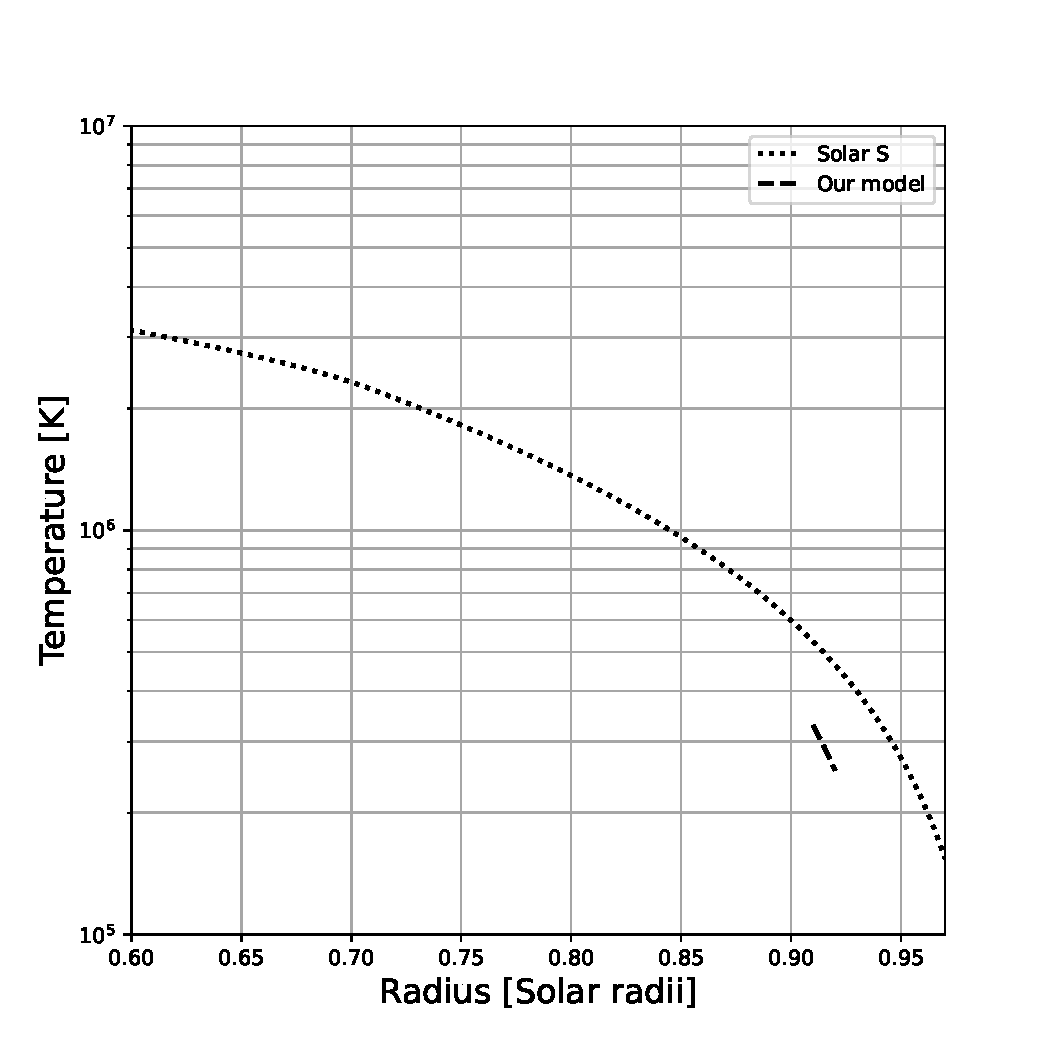
\includegraphics[width=0.8\linewidth]{./solar_vs_model_plots/Temperature.pdf} % Adjust the width as necessary
    \caption{Temperature as a function of radius for the integrated hydrostatic model in dashed lines and the Solar S model in dotted line.}
    \label{fig:temperature} % For referencing the figure elsewhere in your document
\end{figure}

\begin{figure}[htbp]
    \centering
    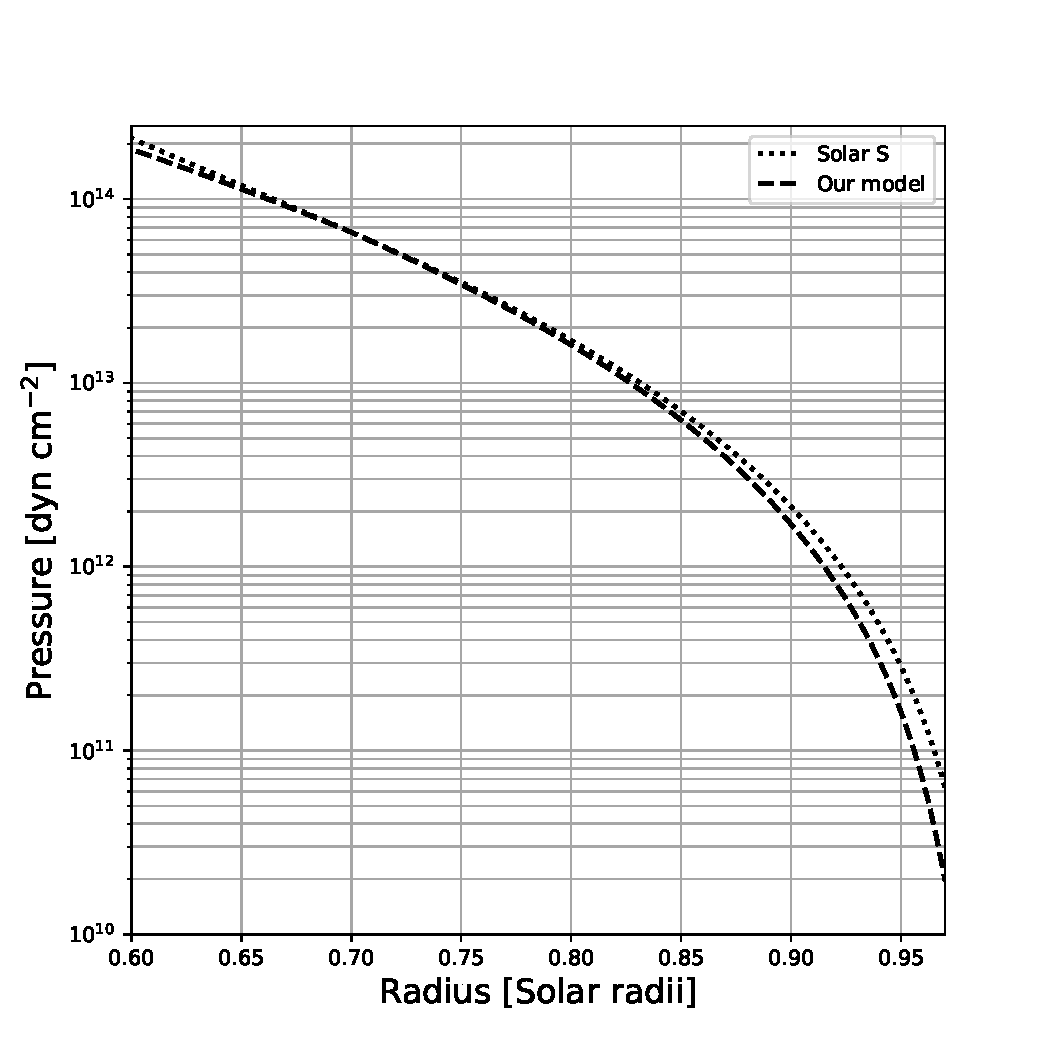
\includegraphics[width=0.8\linewidth]{./solar_vs_model_plots/Pressure.pdf} % Adjust the width as necessary
    \caption{Pressure as a function of radius for the integrated hydrostatic model in dashed lines and the Solar S model in dotted line.}
    \label{fig:pressure} % For referencing the figure elsewhere in your document
\end{figure}

\begin{figure}[htbp]
    \centering
    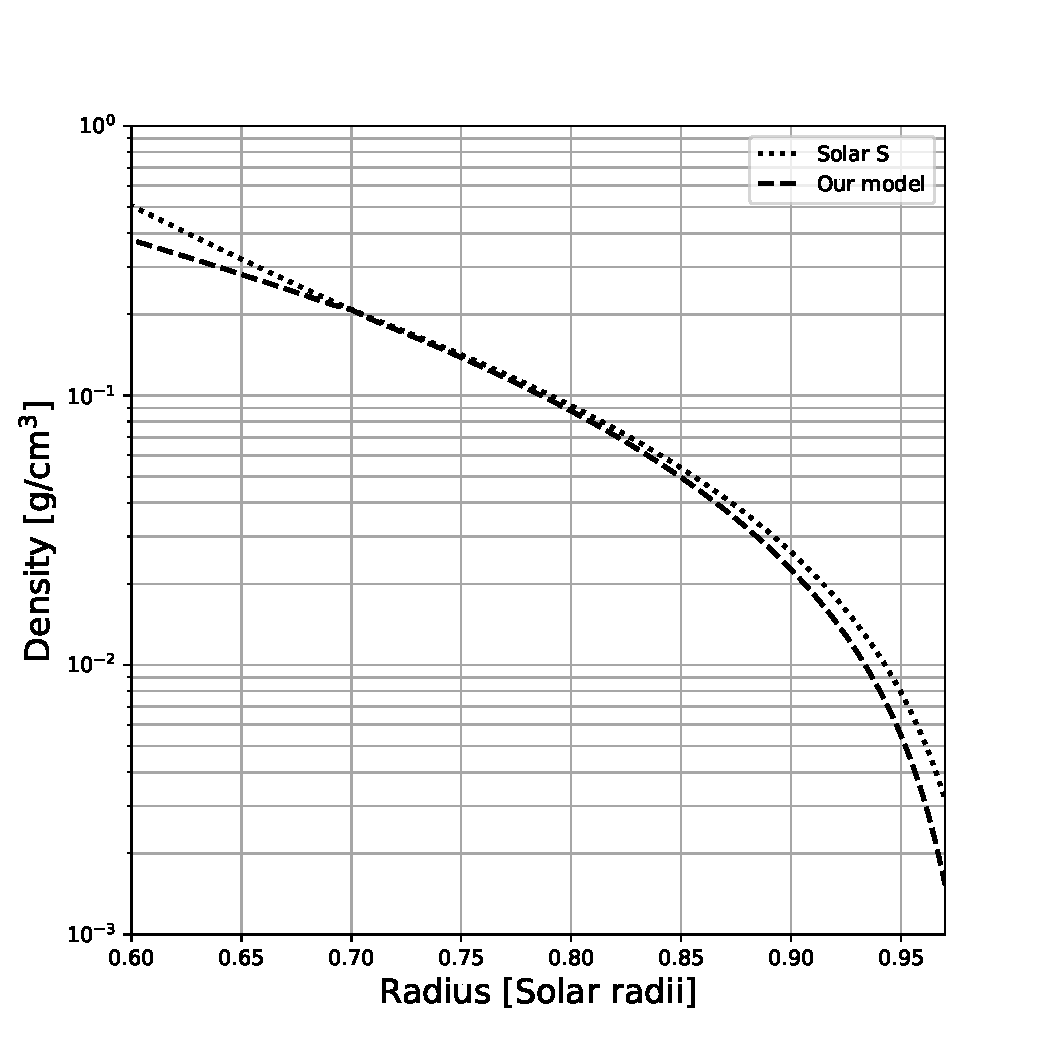
\includegraphics[width=0.8\linewidth]{./solar_vs_model_plots/Density.pdf} % Adjust the width as necessary
    \caption{Density as a function of radius for the integrated hydrostatic model in dashed lines and the Solar S model in dotted line.}
    \label{fig:density} % For referencing the figure elsewhere in your document
\end{figure}

\begin{figure}[htbp]
    \centering
    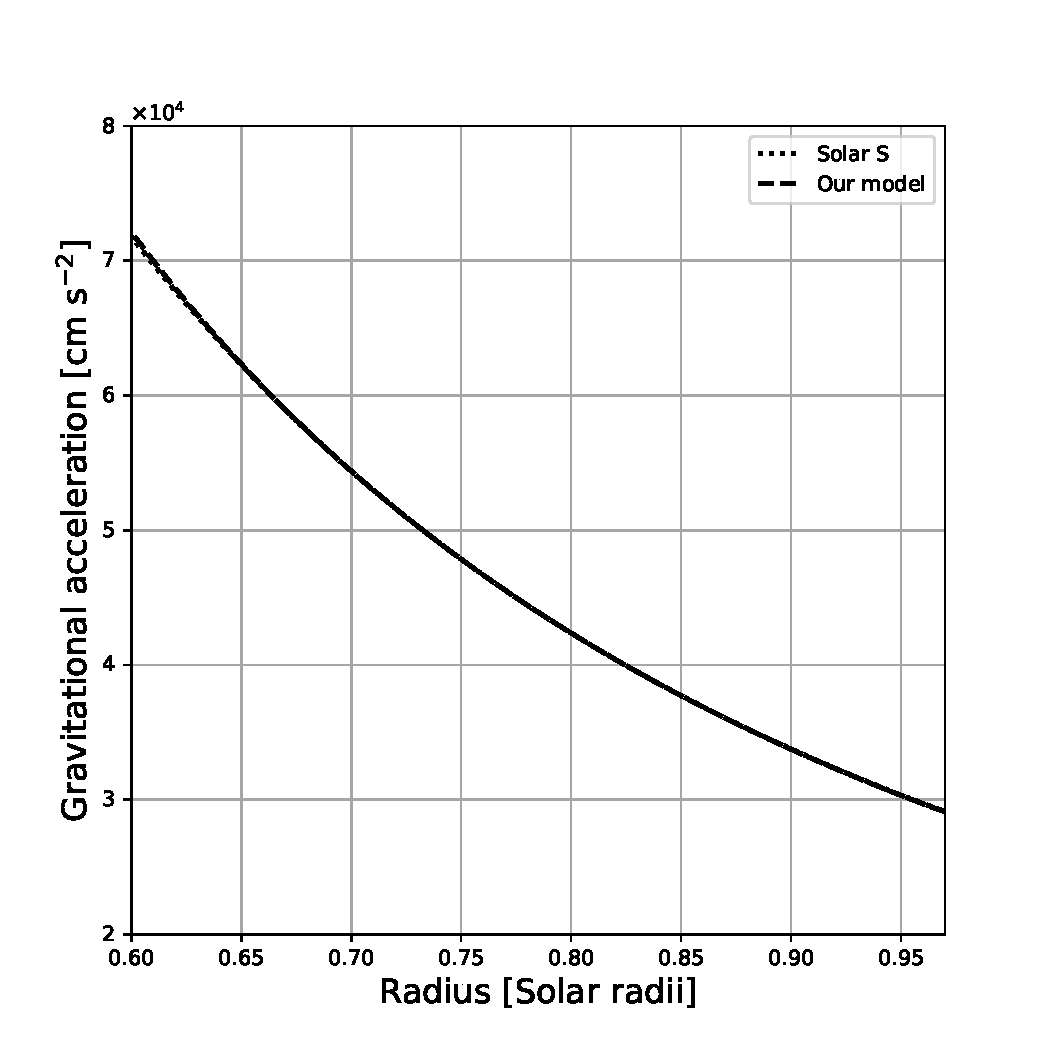
\includegraphics[width=0.8\linewidth]{./solar_vs_model_plots/Gravitational_acceleration.pdf} % Adjust the width as necessary
    \caption{Gravitational acceleration as a function of radius for the integrated hydrostatic model in dashed lines and the Solar S model in dotted line.}
    \label{fig:gravitationa_acceleration} % For referencing the figure elsewhere in your document
\end{figure}

\subsection{Code testing, maybe not in theory}
%\include{cosmology}
%\include{fRgrav}
%\include{bispectrum}
%\include{frame}
%\include{modify}
%\include{results}
%\include{conclusions}
	
\addcontentsline{toc}{part}{\numberline{}Appendicies}
\part*{Appendices}
\appendix
%\include{appendix}

% Include the necessary appendices

\addcontentsline{toc}{chapter}{\numberline{}Bibliography}
\bibliographystyle{unsrt}
\bibliography{refs}
%\bibliography{fRBib}
\end{document}
